\documentclass{standalone}
\usepackage{tikz}
\usetikzlibrary{patterns, positioning}


\begin{document}
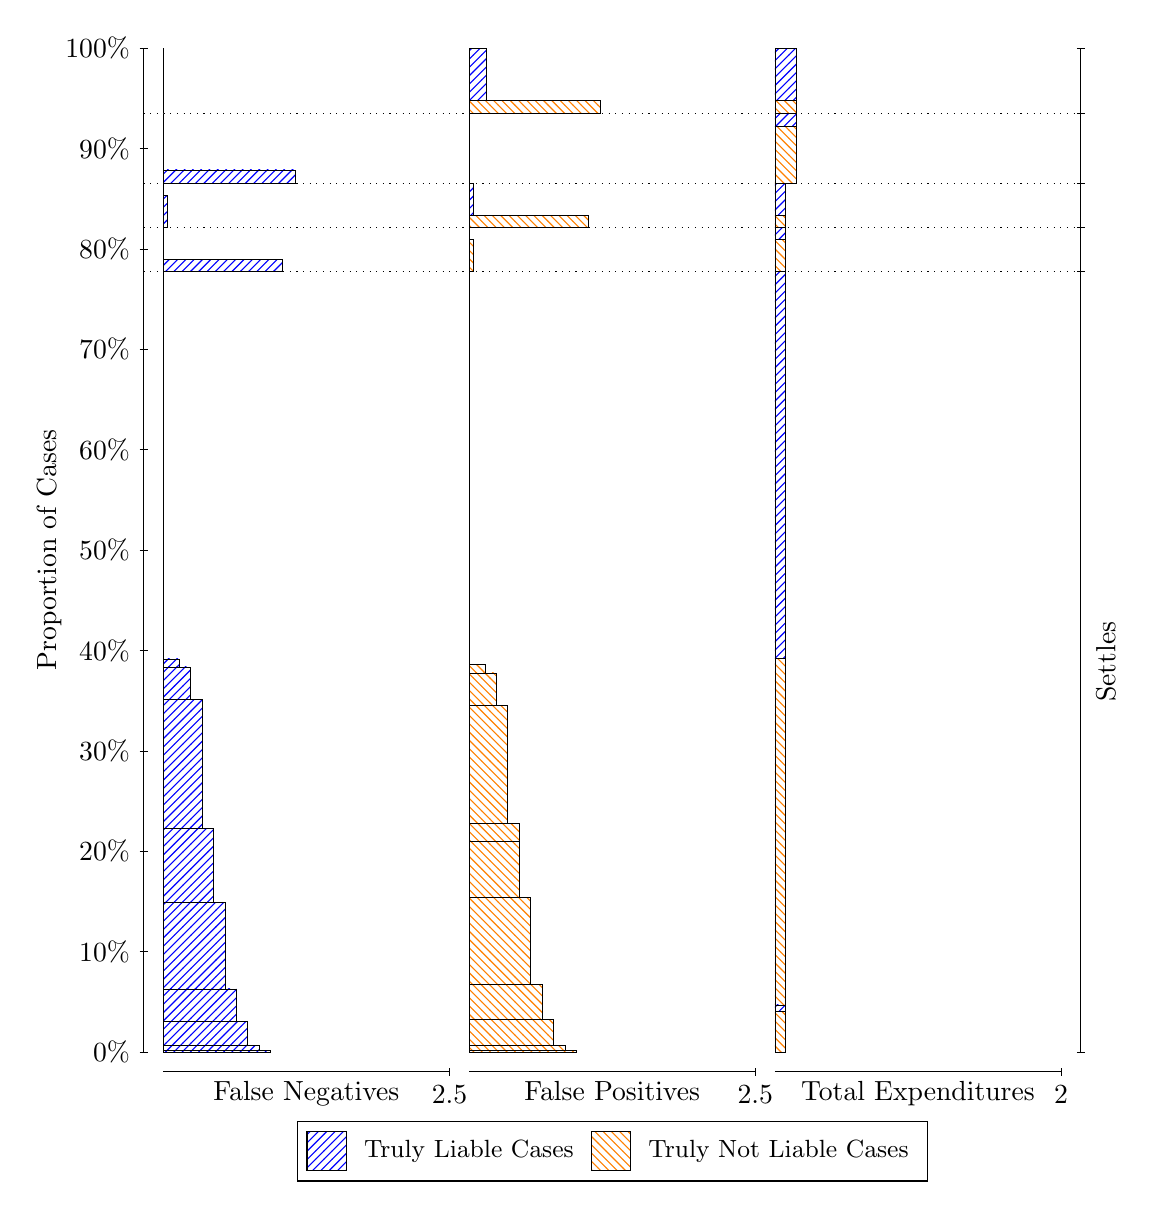
\begin{tikzpicture}
\draw[black, very thin] (1.5,1.75) -- (1.5,14.5);
\node[rotate=90, text=black, anchor=center] at (0.3, 8.125) {Proportion of Cases};
\draw[black, very thin] (1.45,1.75) -- (1.55,1.75);
\node[text=black, anchor=east] at (1.45, 1.75) {0\%};
\draw[black, very thin] (1.45,3.025) -- (1.55,3.025);
\node[text=black, anchor=east] at (1.45, 3.025) {10\%};
\draw[black, very thin] (1.45,4.3) -- (1.55,4.3);
\node[text=black, anchor=east] at (1.45, 4.3) {20\%};
\draw[black, very thin] (1.45,5.575) -- (1.55,5.575);
\node[text=black, anchor=east] at (1.45, 5.575) {30\%};
\draw[black, very thin] (1.45,6.85) -- (1.55,6.85);
\node[text=black, anchor=east] at (1.45, 6.85) {40\%};
\draw[black, very thin] (1.45,8.125) -- (1.55,8.125);
\node[text=black, anchor=east] at (1.45, 8.125) {50\%};
\draw[black, very thin] (1.45,9.4) -- (1.55,9.4);
\node[text=black, anchor=east] at (1.45, 9.4) {60\%};
\draw[black, very thin] (1.45,10.675) -- (1.55,10.675);
\node[text=black, anchor=east] at (1.45, 10.675) {70\%};
\draw[black, very thin] (1.45,11.95) -- (1.55,11.95);
\node[text=black, anchor=east] at (1.45, 11.95) {80\%};
\draw[black, very thin] (1.45,13.225) -- (1.55,13.225);
\node[text=black, anchor=east] at (1.45, 13.225) {90\%};
\draw[black, very thin] (1.45,14.5) -- (1.55,14.5);
\node[text=black, anchor=east] at (1.45, 14.5) {100\%};

\draw[black, very thin] (13.4,1.75) -- (13.4,14.5);
\draw[black, very thin] (13.35,1.75) -- (13.45,1.75);
\node[anchor=west] at (13.35, 1.75) {};
\draw[black, very thin] (13.35,11.665) -- (13.45,11.665);
\node[anchor=west] at (13.35, 11.665) {};
\draw[black, very thin] (13.35,12.22) -- (13.45,12.22);
\node[anchor=west] at (13.35, 12.22) {};
\draw[black, very thin] (13.35,12.783) -- (13.45,12.783);
\node[anchor=west] at (13.35, 12.783) {};
\draw[black, very thin] (13.35,13.67) -- (13.45,13.67);
\node[anchor=west] at (13.35, 13.67) {};
\draw[black, very thin] (13.35,14.5) -- (13.45,14.5);
\node[anchor=west] at (13.35, 14.5) {};

\draw[black, very thin, pattern color=blue, pattern=north east lines] (1.75,1.75) rectangle (3.1125,1.7708);
\draw[black, very thin, pattern color=blue, pattern=north east lines] (1.75,1.7708) rectangle (2.9672,1.8293);
\draw[black, very thin, pattern color=blue, pattern=north east lines] (1.75,1.8293) rectangle (2.8218,2.1344);
\draw[black, very thin, pattern color=blue, pattern=north east lines] (1.75,2.1344) rectangle (2.6765,2.5501);
\draw[black, very thin, pattern color=blue, pattern=north east lines] (1.75,2.5501) rectangle (2.5312,3.6488);
\draw[black, very thin, pattern color=blue, pattern=north east lines] (1.75,3.6488) rectangle (2.3858,4.592);
\draw[black, very thin, pattern color=blue, pattern=north east lines] (1.75,4.592) rectangle (2.2405,6.2278);
\draw[black, very thin, pattern color=blue, pattern=north east lines] (1.75,6.2278) rectangle (2.0952,6.6402);
\draw[black, very thin, pattern color=blue, pattern=north east lines] (1.75,6.6402) rectangle (1.9498,6.7416);
\draw[black, very thin, pattern color=orange, pattern=north west lines] (1.75,6.7416) rectangle (1.75,11.665);
\draw[black, very thin, pattern color=blue, pattern=north east lines] (1.75,11.665) rectangle (3.2578,11.814);
\draw[black, very thin, pattern color=orange, pattern=north west lines] (1.75,11.814) rectangle (1.75,12.22);
\draw[black, very thin, pattern color=blue, pattern=north east lines] (1.75,12.22) rectangle (1.8045,12.624);
\draw[black, very thin, pattern color=orange, pattern=north west lines] (1.75,12.624) rectangle (1.75,12.783);
\draw[black, very thin, pattern color=blue, pattern=north east lines] (1.75,12.783) rectangle (3.4213,12.953);
\draw[black, very thin, pattern color=orange, pattern=north west lines] (1.75,12.953) rectangle (1.75,13.67);
\draw[black, very thin, pattern color=orange, pattern=north west lines] (1.75,13.67) rectangle (1.75,13.839);
\draw[black, very thin, pattern color=blue, pattern=north east lines] (1.75,13.839) rectangle (1.75,14.5);
\draw[black, very thin, pattern color=orange, pattern=north west lines] (5.6333,1.75) rectangle (6.9958,1.7707);
\draw[black, very thin, pattern color=orange, pattern=north west lines] (5.6333,1.7707) rectangle (6.8505,1.8299);
\draw[black, very thin, pattern color=orange, pattern=north west lines] (5.6333,1.8299) rectangle (6.7052,2.1648);
\draw[black, very thin, pattern color=orange, pattern=north west lines] (5.6333,2.1648) rectangle (6.5598,2.609);
\draw[black, very thin, pattern color=orange, pattern=north west lines] (5.6333,2.609) rectangle (6.4145,3.7161);
\draw[black, very thin, pattern color=orange, pattern=north west lines] (5.6333,3.7161) rectangle (6.2692,4.4201);
\draw[black, very thin, pattern color=orange, pattern=north west lines] (5.6333,4.4201) rectangle (6.2692,4.6486);
\draw[black, very thin, pattern color=orange, pattern=north west lines] (5.6333,4.6486) rectangle (6.1238,6.1541);
\draw[black, very thin, pattern color=orange, pattern=north west lines] (5.6333,6.1541) rectangle (5.9785,6.5654);
\draw[black, very thin, pattern color=orange, pattern=north west lines] (5.6333,6.5654) rectangle (5.8332,6.6734);
\draw[black, very thin, pattern color=blue, pattern=north east lines] (5.6333,6.6734) rectangle (5.6333,11.665);
\draw[black, very thin, pattern color=orange, pattern=north west lines] (5.6333,11.665) rectangle (5.6878,12.071);
\draw[black, very thin, pattern color=blue, pattern=north east lines] (5.6333,12.071) rectangle (5.6333,12.22);
\draw[black, very thin, pattern color=orange, pattern=north west lines] (5.6333,12.22) rectangle (7.1412,12.379);
\draw[black, very thin, pattern color=blue, pattern=north east lines] (5.6333,12.379) rectangle (5.6878,12.783);
\draw[black, very thin, pattern color=orange, pattern=north west lines] (5.6333,12.783) rectangle (5.6333,13.5);
\draw[black, very thin, pattern color=blue, pattern=north east lines] (5.6333,13.5) rectangle (5.6333,13.67);
\draw[black, very thin, pattern color=orange, pattern=north west lines] (5.6333,13.67) rectangle (7.3047,13.839);
\draw[black, very thin, pattern color=blue, pattern=north east lines] (5.6333,13.839) rectangle (5.8513,14.5);
\draw[black, very thin, pattern color=orange, pattern=north west lines] (9.5167,1.75) rectangle (9.6529,2.2693);
\draw[black, very thin, pattern color=blue, pattern=north east lines] (9.5167,2.2693) rectangle (9.6529,2.3486);
\draw[black, very thin, pattern color=orange, pattern=north west lines] (9.5167,2.3486) rectangle (9.6529,6.7527);
\draw[black, very thin, pattern color=blue, pattern=north east lines] (9.5167,6.7527) rectangle (9.6529,11.665);
\draw[black, very thin, pattern color=orange, pattern=north west lines] (9.5167,11.665) rectangle (9.6529,12.071);
\draw[black, very thin, pattern color=blue, pattern=north east lines] (9.5167,12.071) rectangle (9.6529,12.22);
\draw[black, very thin, pattern color=orange, pattern=north west lines] (9.5167,12.22) rectangle (9.6529,12.379);
\draw[black, very thin, pattern color=blue, pattern=north east lines] (9.5167,12.379) rectangle (9.6529,12.783);
\draw[black, very thin, pattern color=orange, pattern=north west lines] (9.5167,12.783) rectangle (9.7892,13.5);
\draw[black, very thin, pattern color=blue, pattern=north east lines] (9.5167,13.5) rectangle (9.7892,13.67);
\draw[black, very thin, pattern color=orange, pattern=north west lines] (9.5167,13.67) rectangle (9.7892,13.839);
\draw[black, very thin, pattern color=blue, pattern=north east lines] (9.5167,13.839) rectangle (9.7892,14.5);
\draw[black, dotted] (1.5,11.665) -- (13.4,11.665);
\draw[black, dotted] (1.5,12.22) -- (13.4,12.22);
\draw[black, dotted] (1.5,12.783) -- (13.4,12.783);
\draw[black, dotted] (1.5,13.67) -- (13.4,13.67);
\draw[black, very thin] (1.75,1.5) -- (5.3833,1.5);
\node[text=black, anchor=north] at (3.5667, 1.5) {False Negatives};
\draw[black, very thin] (5.3833,1.45) -- (5.3833,1.55);
\node[text=black, anchor=north] at (5.3833, 1.45) {2.5};

\draw[black, very thin] (5.6333,1.5) -- (9.2667,1.5);
\node[text=black, anchor=north] at (7.45, 1.5) {False Positives};
\draw[black, very thin] (9.2667,1.45) -- (9.2667,1.55);
\node[text=black, anchor=north] at (9.2667, 1.45) {2.5};

\draw[black, very thin] (9.5167,1.5) -- (13.15,1.5);
\node[text=black, anchor=north] at (11.333, 1.5) {Total Expenditures};
\draw[black, very thin] (13.15,1.45) -- (13.15,1.55);
\node[text=black, anchor=north] at (13.15, 1.45) {2};

\node[text=black, centered, rotate=90] at (13.72, 6.7075) {Settles};





\draw (7.449999999999999,1.5) node[draw=none] (baseCoordinate) {};
\begin{scope}[align=center]
        \matrix[scale=0.5, draw=black, below=0.5cm of baseCoordinate, nodes={draw}, column sep=0.1cm]{
            \node[rectangle, draw, minimum width=0.5cm, minimum height=0.5cm, pattern color=blue, pattern=north east lines] {}; &
            \node[draw=none, font=\small, text=black] (B) {Truly Liable Cases}; &
            \node[rectangle, draw, minimum width=0.5cm, minimum height=0.5cm, pattern color=orange, pattern=north west lines] {}; &
            \node[draw=none, font=\small, text=black] (B) {Truly Not Liable Cases}; \\
            };
\end{scope}

\end{tikzpicture}
\end{document}